%%%%%%%%%%%%%%%%%%%%%%%%%%%%%%%%%%%%%%%%%%%%%%%%%%%%%%%%%%%%%%%%%%%%%%%%%%%%%%%%%%
\begin{frame}[fragile]\frametitle{}
\begin{center}
{\Large KNN}
\end{center}
\end{frame}

%%%%%%%%%%%%%%%%%%%%%%%%%%%%%%%%%%%%%%%%%%%%%%%%%%%%%%%%%%
\begin{frame}[fragile]\frametitle{K-Nearest Neighbors (KNN)}
\begin{itemize}
\item Supervised Classification.
\item Algorithm stores all available cases and classifies new cases by a majority vote of its k neighbors. 
\end{itemize}
\end{frame}

%%%%%%%%%%%%%%%%%%%%%%%%%%%%%%%%%%%%%%%%%%%%%%%%%%%%%%%%%%
\begin{frame}[fragile]\frametitle{K-Nearest Neighbors (KNN)}
\begin{itemize}
\item ``A man is known by the company he keeps''
\item KNN can easily be mapped to our real lives. If you want to learn about a person, of whom you have no information, you might like to find out about his close friends and the circles he moves in and gain access to his/her information!
\end{itemize}
\end{frame}

%%%%%%%%%%%%%%%%%%%%%%%%%%%%%%%%%%%%%%%%%%%%%%%%%%%%%%%%%%
\begin{frame}[fragile]\frametitle{Intuition for kNN}
\adjustbox{valign=t}{
\begin{minipage}{0.45\linewidth}
\begin{itemize}
\item Set of points (x,y) and two classes (red/blue)
\item Is the box red or blue?
\item How did you guess? By Decision Tree? or by SVM?
\item You saw, nearby points are red.
\end{itemize}

\end{minipage}
}
\hfill
\adjustbox{valign=t}{
\begin{minipage}{0.45\linewidth}
\begin{center}
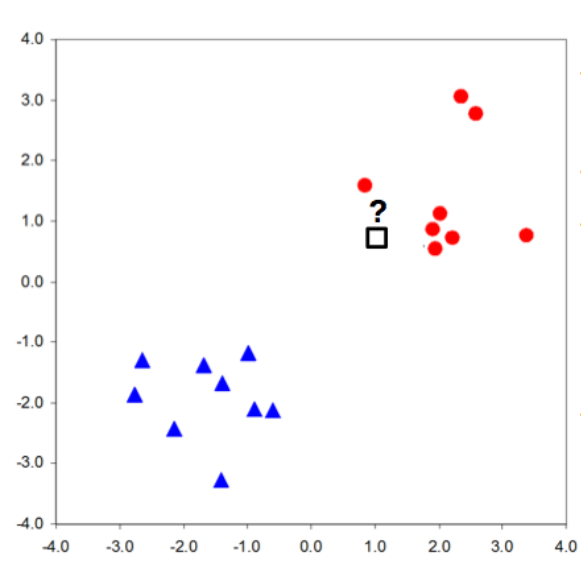
\includegraphics[width=\linewidth,keepaspectratio]{knn5}
\end{center}

\end{minipage}
}
Neighborhood is the basis of KNN.
\end{frame}

%%%%%%%%%%%%%%%%%%%%%%%%%%%%%%%%%%%%%%%%%%%%%%%%%%%%%%%%%%
\begin{frame}[fragile]\frametitle{Nearest-neighbor classification }
\adjustbox{valign=t}{
\begin{minipage}{0.5\linewidth}
\begin{itemize}
\item Use the intuition to classify a new point x: find the most similar training example  x'; predict its class y' 
\item This is true for all the points shown in blue patch/cell.
\item Every training example is going to have a small cell around it.
\item All cells together are called as Voronoi Diagram.
\item Examples: Post office region demarcation, Utility stations, etc.
\end{itemize}
\end{minipage}
}
\hfill
\adjustbox{valign=t}{
\begin{minipage}{0.4\linewidth}
\begin{center}
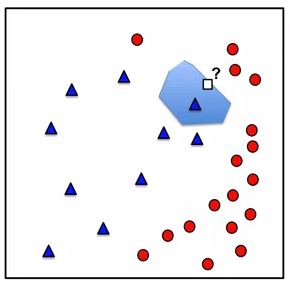
\includegraphics[width=\linewidth,keepaspectratio]{knn15}
\end{center}

\end{minipage}
}
\end{frame}

%%%%%%%%%%%%%%%%%%%%%%%%%%%%%%%%%%%%%%%%%%%%%%%%%%%%%%%%%%
\begin{frame}[fragile]\frametitle{Nearest-neighbor classification }
\adjustbox{valign=t}{
\begin{minipage}{0.5\linewidth}
\begin{itemize}
\item Each cell is such that points in it are closer to its owner Centroid than any other Centroids.
\item Each cell corresponds to a training example.
\item Classification boundary separates the cells based on classes
\item See how a Non-linear complex partitioning is possible, than just linear or margin separation
\end{itemize}
\end{minipage}
}
\hfill
\adjustbox{valign=t}{
\begin{minipage}{0.4\linewidth}
\begin{center}
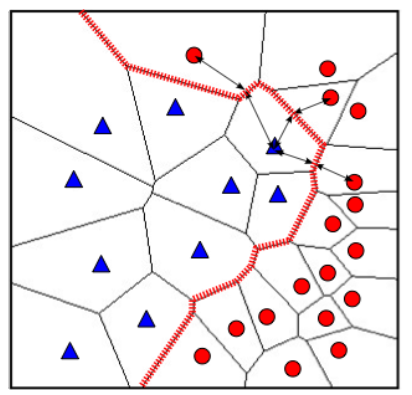
\includegraphics[width=\linewidth,keepaspectratio]{knn6}
\end{center}

\end{minipage}
}
\end{frame}

%%%%%%%%%%%%%%%%%%%%%%%%%%%%%%%%%%%%%%%%%%%%%%%%%%%%%%%%%%
\begin{frame}[fragile]\frametitle{Nearest-neighbor classification }
Limitations

\adjustbox{valign=t}{
\begin{minipage}{0.5\linewidth}
\begin{itemize}
\item But, if you have a Outlier, say the red shown, then whole classification goes for a toss.
\item Boundary becomes too complicated.
\item So, Sensitive to Outliers.
\item Remedy: to look at more than one neighbors to classify yourself.
\item Majority Voting. Adds stability.
\end{itemize}
\end{minipage}
}
\hfill
\adjustbox{valign=t}{
\begin{minipage}{0.4\linewidth}
\begin{center}
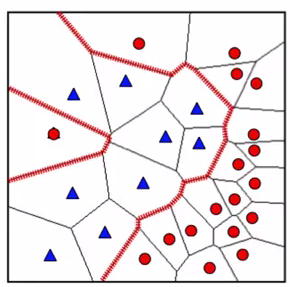
\includegraphics[width=\linewidth,keepaspectratio]{knn16}
\end{center}

\end{minipage}
}
\end{frame}

%%%%%%%%%%%%%%%%%%%%%%%%%%%%%%%%%%%%%%%%%%%%%%%%%%%%%%%%%%
\begin{frame}[fragile]\frametitle{Scaling Issues}
\begin{itemize}
\item Attributes may have to be scaled to prevent distance measures from being dominated by one of the attributes
\item Example, with three dimensions
\begin{itemize}
\item  height of a person may vary from 1.5m to 1.8m
\item   weight of a person may vary from 90lb to 300lb
\item   income of a person may vary from \$10K to \$1M
\end{itemize}
\item Income will dominate if these variables aren't standardized.
\end{itemize}
\end{frame}

%%%%%%%%%%%%%%%%%%%%%%%%%%%%%%%%%%%%%%%%%%%%%%%%%%%%%%%%%%
\begin{frame}[fragile]\frametitle{Standardization}
\begin{itemize}
\item Treat all features ``equally'' so that one feature doesn't dominate the others
\item Common treatment to all variables
\begin{itemize}
\item  Standardize each variable: Mean = 0, Standard Deviation = 1
\item Normalize each variable: Max = 1, Min = 0
\end{itemize}
\end{itemize}
\end{frame}

%%%%%%%%%%%%%%%%%%%%%%%%%%%%%%%%%%%%%%%%%%%%%%%%%%%%%%%%%%%%%%%%%%%%%%%%%%%%%%%%%%
\begin{frame}[fragile]\frametitle{}
\begin{center}
{\Large KNN Algorithm}
\end{center}
\end{frame}

%%%%%%%%%%%%%%%%%%%%%%%%%%%%%%%%%%%%%%%%%%%%%%%%%%%%%%%%%%
\begin{frame}[fragile]\frametitle{Classification Algorithm}
\begin{itemize}
\item Given: training examples $(x_i,y_i)$ and test point $x$ to classify.
\item Here, there is no traditional training phase, where model is built.
\item Compute distance $D(x,x_i)$ to every training example $x_i $
\item Select $k$ closest instances $x_{i1} \ldots x_{ik}$ and their labels $y_{i1} \ldots y_{ik}$
\item Output the class $y*$ which is most frequent in $y_{i1} \ldots y_{ik}$
\end{itemize}
\end{frame}


%%%%%%%%%%%%%%%%%%%%%%%%%%%%%%%%%%%%%%%%%%%%%%%%%%%%%%%%%%
\begin{frame}[fragile]\frametitle{KNN as Regression}
\begin{itemize}
\item Given: training examples $(x_i,y_i)$ with $y_i$ as real valued, like profits, price, etc. and test point $x$ to predict the target value.
\item Here is no traditional training phase, where model is built.
\item Compute distance $D(x,x_i)$ to every training example $x_i $
\item Select $k$ closest instances $x_{i1} \ldots x_{ik}$ and their labels $y_{i1} \ldots y_{ik}$
\item Output the target $y*$ which is MEAN of $y_{i1} \ldots y_{ik}$
\end{itemize}
\end{frame}

%%%%%%%%%%%%%%%%%%%%%%%%%%%%%%%%%%%%%%%%%%%%%%%%%%%%%%%%%%
\begin{frame}[fragile]\frametitle{KNN Regression Example: 1d}
\begin{itemize}
\item Given:Some set of points $(x_i,y_i)$. The function/relation between them is unknown.
\item Goal: given, unseen x, find its y value.
\end{itemize}
\begin{center}
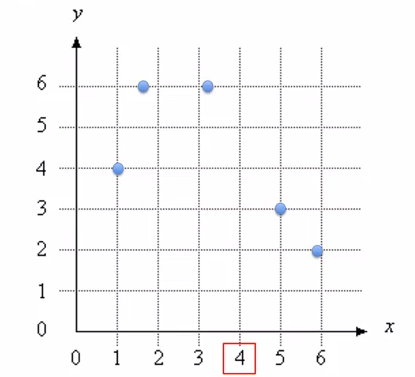
\includegraphics[width=0.4\linewidth,keepaspectratio]{knn19}
\end{center}
\end{frame}

%%%%%%%%%%%%%%%%%%%%%%%%%%%%%%%%%%%%%%%%%%%%%%%%%%%%%%%%%%
\begin{frame}[fragile]\frametitle{KNN Regression Example: 1d}
\begin{itemize}
\item Who are the neighbours of $x=4$ on x axis?
\item If we want only one nearest neighbour (1-NN) then 3.2 is nearest, its y is 6, so thats the final prediction for $x=4$.
\end{itemize}
\begin{center}
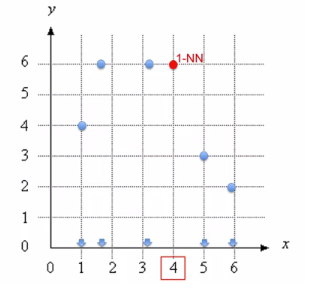
\includegraphics[width=0.4\linewidth,keepaspectratio]{knn20}
\end{center}
\end{frame}


%%%%%%%%%%%%%%%%%%%%%%%%%%%%%%%%%%%%%%%%%%%%%%%%%%%%%%%%%%
\begin{frame}[fragile]\frametitle{KNN Regression Example: 1d}
\begin{itemize}
\item If we find 2-NN then 3.2 and 5 are the neighbours
\item Their ys are 6 and 3.
\item Avereage of theose ys is 4.5. So for $x=4$, y is predicted as 4.5
\end{itemize}
\begin{center}
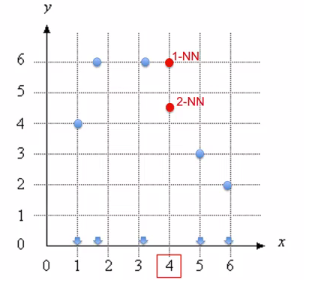
\includegraphics[width=0.4\linewidth,keepaspectratio]{knn21}
\end{center}
\end{frame}


%%%%%%%%%%%%%%%%%%%%%%%%%%%%%%%%%%%%%%%%%%%%%%%%%%%%%%%%%%
\begin{frame}[fragile]\frametitle{KNN Regression Example: 1d}
\begin{itemize}
\item Its easy to see that if you go on adding neighbours, you may not be more accurate all the time.
\item If you take all the neighbours?
\item As it is just avarage of those many y values aorund.
\item Is that good? No. There is one sweet spot (tradeoff).
\end{itemize}
\begin{center}
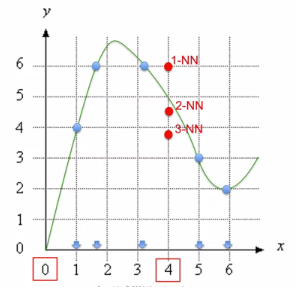
\includegraphics[width=0.4\linewidth,keepaspectratio]{knn22}
\end{center}
\end{frame}


%%%%%%%%%%%%%%%%%%%%%%%%%%%%%%%%%%%%%%%%%%%%%%%%%%%%%%%%%%
\begin{frame}[fragile]\frametitle{KNN Regression Example: 1d}
\begin{itemize}
\item So, if you are in the middle, then  its intrapolation, works.
\item If you are at boundaries then, its hard to predict. Extrapolation
\item Find for $x=0$ with 1-NN, 2NN.
\end{itemize}
\end{frame}

%%%%%%%%%%%%%%%%%%%%%%%%%%%%%%%%%%%%%%%%%%%%%%%%%%%
\begin{frame}[fragile] \frametitle{Choosing the right k}
%
%\adjustbox{valign=t}{
%\begin{minipage}{0.45\linewidth}
\begin{itemize}
\item Say, we are classifying middle point, into either +s or -s
\item Depending on k (ie number of neighbours), it may get classified as + or -
\item Say if k is upto 5, then it would be +, if say,20 then it would be -ve

\end{itemize}

%\end{minipage}
%}
%\hfill
%\adjustbox{valign=t}{
%\begin{minipage}{0.45\linewidth}
\begin{center}
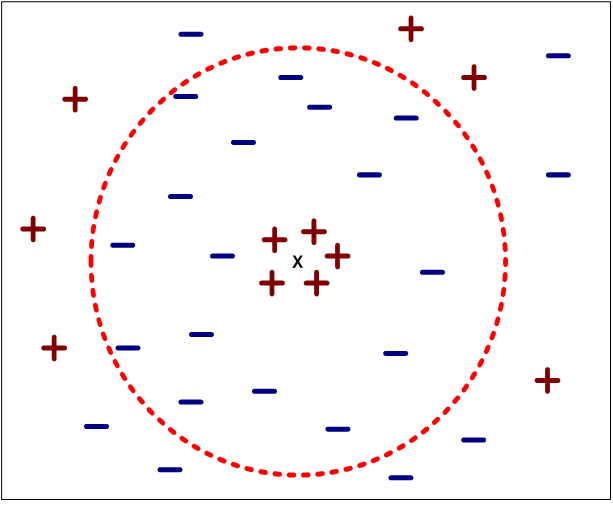
\includegraphics[width=0.5\linewidth,keepaspectratio]{rightk}
\end{center}
%
%\end{minipage}
%}
\end{frame}


%%%%%%%%%%%%%%%%%%%%%%%%%%%%%%%%%%%%%%%%%%%%%%%%%%%
\begin{frame}[fragile] \frametitle{Choosing the right k}
%
%\adjustbox{valign=t}{
%\begin{minipage}{0.45\linewidth}
\begin{itemize}
\item If k is too small, sensitive to noise points in the training data
\item Susceptible to overfitting
\item If k is too large, neighborhood may include points from other classes
\item Susceptible to misclassification

\end{itemize}

%\end{minipage}
%}
%\hfill
%\adjustbox{valign=t}{
%\begin{minipage}{0.45\linewidth}
\begin{center}
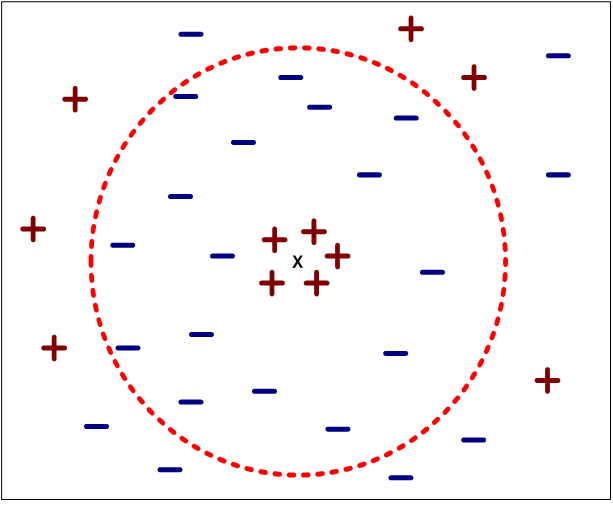
\includegraphics[width=0.5\linewidth,keepaspectratio]{rightk}
\end{center}
%
%\end{minipage}
%}
\end{frame}

%%%%%%%%%%%%%%%%%%%%%%%%%%%%%%%%%%%%%%%%%%%%%%%%%%%%%%%%%%
\begin{frame}[fragile] \frametitle{Choosing the right k}
\begin{itemize}
\item Do, cross validation.
\item Take validation set out of training set. Make it separate, not part of Training set any more.
\item Try different k's on the validation set.
\item You will predict y for evey x in the test set.
\item As you know the correct labels, see which k gives best result.
\end{itemize}
\end{frame}

%%%%%%%%%%%%%%%%%%%%%%%%%%%%%%%%%%%%%%%%%%%%%%%%%%%%%%%%%%%%%%%%%%%%%%%%%%%%%%%%%%
\begin{frame}[fragile]\frametitle{}
\begin{center}
{\Large Similarity Criterion - Distance}
\end{center}
\end{frame}


%%%%%%%%%%%%%%%%%%%%%%%%%%%%%%%%%%%%%%%%%%%%%%%%%%%%%%%%%%
\begin{frame}[fragile]\frametitle{Distance measures }
\begin{itemize}
\item Crucial component
\item Finds similarity value between two data points.
\item Types: Euclidean (for floats), Hamming (for enums), Minkowski (general form)
\end{itemize}
\end{frame}

%%%%%%%%%%%%%%%%%%%%%%%%%%%%%%%%%%%%%%%%%%%%%%%%%%%%%%%%%%
\begin{frame}[fragile]\frametitle{Distances}
\begin{itemize}
\item The case being assigned to the class is most common among its K nearest neighbors measured by a distance
function.
\item These distance functions can be Euclidean, Manhattan, Minkowski and Hamming distance.
\end{itemize}
%\begin{center}
%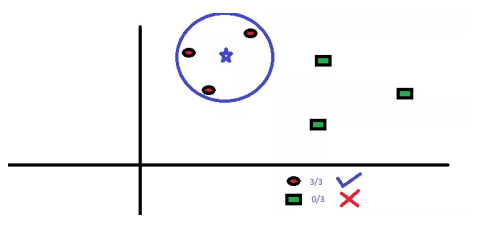
\includegraphics[width=0.7\linewidth,keepaspectratio]{knn}
%\end{center}
\end{frame}

%%%%%%%%%%%%%%%%%%%%%%%%%%%%%%%%%%%%%%%%%%%%%%%%%%%%%%%%%%
\begin{frame}[fragile]\frametitle{Example}
\begin{itemize}
\item Handwritten digit recognition
\item $16 \times 16$ bitmaps
\item Euclidean Distance over pixels between testing bitmap A and training bitmap B. $D(A,B) = \sqrt{\sum_r \sum_c (A_{r,c} - B_{r,c})^2}$
\item Find 7 nearest training examples, their known digit labels. 
\item Find most occurring among those labels
\end{itemize}
\begin{center}
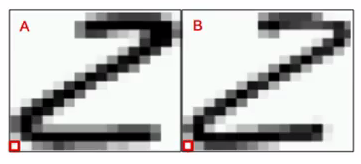
\includegraphics[width=0.5\linewidth,keepaspectratio]{knn17}
\end{center}
\end{frame}

%%%%%%%%%%%%%%%%%%%%%%%%%%%%%%%%%%%%%%%%%%%%%%%%%%%%%%%%%%
\begin{frame}[fragile]\frametitle{Example}
\begin{center}
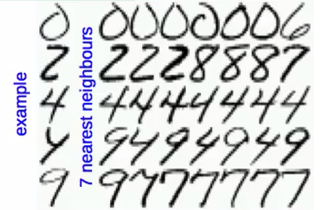
\includegraphics[width=0.4\linewidth,keepaspectratio]{knn18}
\end{center}
\begin{itemize}
\item For ``0'', max vote goes to ``0''.
\item For ``2'', there is a tie, may add more neighbors to decide.
\item For ``4'', things may fail.
\item Simple algorithm, but impressive results. 
\item Accuracy:
\begin{itemize}
\item 7-NN: 95.2\%
\item SVM: 95.8\%
\item Humans: 97.5\%, Humans are not perfect either!!
\end{itemize}
\end{itemize}
\end{frame}

%%%%%%%%%%%%%%%%%%%%%%%%%%%%%%%%%%%%%%%%%%%%%%%%%%%%%%%%%%
\begin{frame}[fragile]\frametitle{Distance measures  (Recap)}
\begin{itemize}
\item Euclidean is for numerical features: $\sqrt{\sum (x_d - x'_d)^2}$
\item Hamming is for categorical features: $\sum 1_{x_d \neq x'_d}$ ie  number of attributes, where $x, x'$  differ 
\item Minkowski distance:  $p\sqrt{\sum (x_d - x'_d)^p}$
	\begin{itemize}
	\item p = 2: Euclidean 
	\item p = 1: Manhattan
	\item p = 0: Hamming 
	\end{itemize}
\end{itemize}
\end{frame}

%%%%%%%%%%%%%%%%%%%%%%%%%%%%%%%%%%%%%%%%%%%%%%%%%%%%%%%%%%%%%%%%%%%%%%%%%%%%%%%%%%
\begin{frame}[fragile]\frametitle{}
\begin{center}
{\Large Implementing KNN}
\end{center}
\end{frame}


%%%%%%%%%%%%%%%%%%%%%%%%%%%%%%%%%%%%%%%%%%%%%%%%%%%%%%%%%%
\begin{frame}[fragile]\frametitle{Writing our Own KNN from Scratch}
A machine learning algorithm usually consists of 2 main steps:

\begin{itemize}
\item  A training step that takes as input the training data X and the corresponding target y and outputs a learned model h
\item A predict step that takes as input new and unseen observations and uses the function h
to output their corresponding responses.
\end{itemize}
\end{frame}

%%%%%%%%%%%%%%%%%%%%%%%%%%%%%%%%%%%%%%%%%%%%%%%%%%%%%%%%%%
\begin{frame}[fragile]\frametitle{Writing our Own KNN from Scratch}
In the case of KNN, which as discussed earlier, is a lazy algorithm, the training block reduces to just memorizing the training data
\begin{lstlisting}
def train(X_train, y_train):
	# do nothing 
	return
\end{lstlisting}
\end{frame}

%%%%%%%%%%%%%%%%%%%%%%%%%%%%%%%%%%%%%%%%%%%%%%%%%%%%%%%%%%
\begin{frame}[fragile]\frametitle{Writing our Own KNN from Scratch}
Now we need to write the predict method which must do the following:
\begin{itemize}
\item  It needs to compute the euclidean distance between the ``new'' observation and all the data points in the training set. 
\item It must then select the K nearest ones and perform a majority vote. 
\item It then assigns the corresponding label to the observation. 
\end{itemize}
\end{frame}

%%%%%%%%%%%%%%%%%%%%%%%%%%%%%%%%%%%%%%%%%%%%%%%%%%%%%%%%%%
\begin{frame}[fragile]\frametitle{Writing our Own KNN from Scratch}
\begin{lstlisting}
def predict(X_train, y_train, x_test, k):
	distances = []
	targets = []

	for i in range(len(X_train)):

		distance = np.sqrt(np.sum(np.square(x_test - 
		                                            X_train[i, :])))
		distances.append([distance, i])

	distances = sorted(distances)

	for i in range(k):
		index = distances[i][1]
		targets.append(y_train[index])

	return Counter(targets).most_common(1)[0][0]
\end{lstlisting}
\end{frame}

%%%%%%%%%%%%%%%%%%%%%%%%%%%%%%%%%%%%%%%%%%%%%%%%%%%%%%%%%%
\begin{frame}[fragile]\frametitle{Writing our Own KNN from Scratch}
Putting it all together, we can define the function KNearestNeighbor, which loops over every test example and makes a prediction.
\begin{lstlisting}
def kNearestNeighbor(X_train,y_train,X_test, predictions, k):
	train(X_train, y_train)

	for i in range(len(X_test)):
		predictions.append(predict(X_train, y_train, 
		                                            X_test[i, :], k))
\end{lstlisting}
\end{frame}

%%%%%%%%%%%%%%%%%%%%%%%%%%%%%%%%%%%%%%%%%%%%%%%%%%%%%%%%%%
\begin{frame}[fragile]\frametitle{Writing our Own KNN from Scratch}
Let's go ahead and run our algorithm
\begin{lstlisting}
# making our predictions 
predictions = []

kNearestNeighbor(X_train, y_train, X_test, predictions, 7)

# transform the list into an array
predictions = np.asarray(predictions)

# evaluating accuracy
accuracy = accuracy_score(y_test, predictions)
print('\nThe accuracy is %d%%' % accuracy*100)
\end{lstlisting}
\end{frame}


%%%%%%%%%%%%%%%%%%%%%%%%%%%%%%%%%%%%%%%%%%%%%%%%%%%%%%%%%%
\begin{frame}[fragile]\frametitle{Optimizing KNN}
\begin{itemize}
\item  Comparing a query point a in d dimensions against n training examples computes with a runtime of $O(nd)$, which can cause lag as points reach millions or billions. 
\item Popular choices to speed up KNN include:
\begin{itemize}
\item  Vernoi Diagrams: partitioning plane into regions
based on distance to points in a specific subset of
the plane
\item  Grid Indexes: carve up space into d-dimensional
boxes or grids and calculate the NN in the same cell
as the point
\item  Locality Sensitive Hashing (LSH): abandons
the idea of finding the exact nearest neighbors. In-
stead, batch up nearby points to quickly find the
most appropriate bucket B for our query point.
\end{itemize}
\end{itemize}
\end{frame}

%
%
%
%%%%%%%%%%%%%%%%%%%%%%%%%%%%%%%%%%%%%%%%%%%%%%%%%%%%%%%%%%%
%\begin{frame}[fragile]\frametitle{Classifying not Clustering}
%To classify an unknown record
%\begin{itemize}
%\item Compute distance to other training records
%\item Identify k nearest neighbors 
%\item Use class labels of nearest neighbors to determine the class label of unknown record (e.g., by taking majority vote)
%\end{itemize}
%\begin{center}
%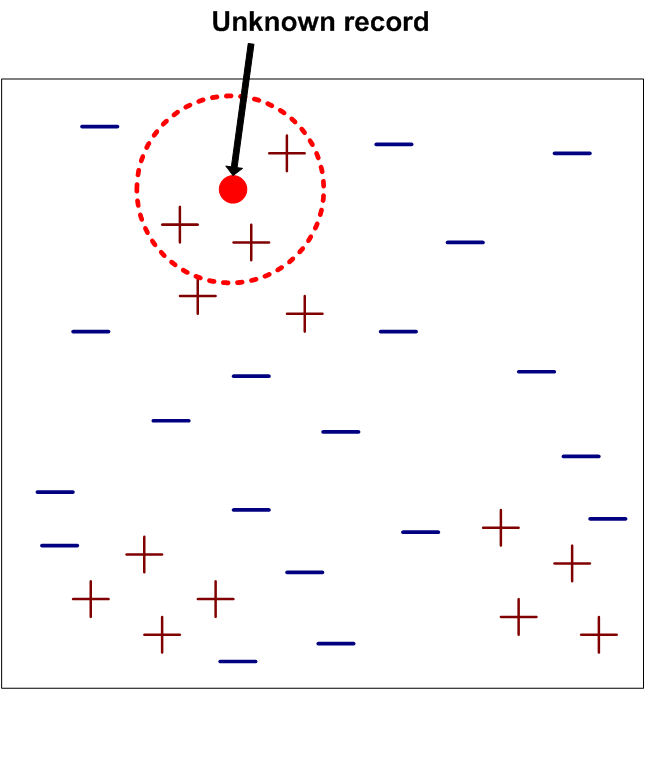
\includegraphics[width=0.35\linewidth,keepaspectratio]{kunknown}
%\end{center}
%\end{frame}
%


%%%%%%%%%%%%%%%%%%%%%%%%%%%%%%%%%%%%%%%%%%%%%%%%%%%%%%%%%%%
%\begin{frame}[fragile]\frametitle{Definition}
%The k-nearest neighbors of a given example x are the k points that are closest to x
%\begin{itemize}
%\item Classification changes depending on the chosen k
%\item Majority Voting
%\item Tie Scenario: Randomly choose classification?  For binary problems, usually an odd k is used to avoid ties.
%\end{itemize}
%\begin{center}
%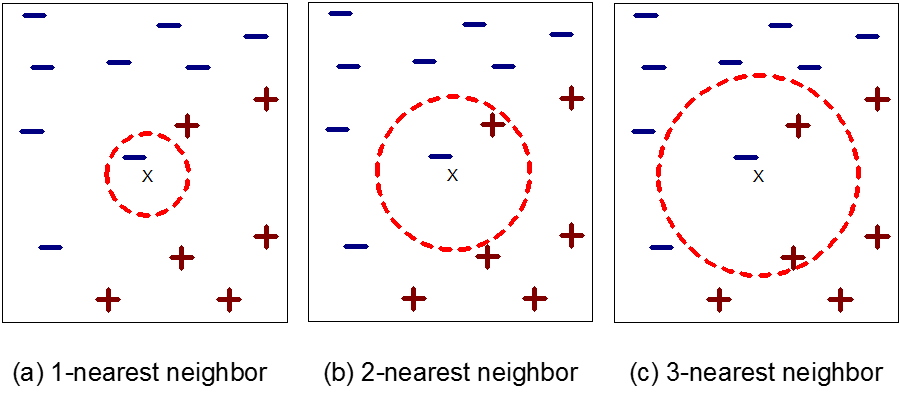
\includegraphics[width=0.6\linewidth,keepaspectratio]{knearest}
%\end{center}
%\end{frame}
%
%
%
%%%%%%%%%%%%%%%%%%%%%%%%%%%%%%%%%%%%%%%%%%%%%%%%%%%%%%%%%%%
%\begin{frame}[fragile]\frametitle{How to Choose Initial Centroids?}
%\begin{itemize}
%\item One strategy: choose the k Centroids at random
%\item Different runs of k-means on same data:
%	\begin{itemize}
%	\item Will produce different iterations (because the starting clusters are different)
%	\item May produce different final clusters
%	\end{itemize}
%\item Most convergence happens in the first few iterations
%\item Sometimes the termination condition is:
%``repeat until only 1\% of the points change clusters''
%\end{itemize}
%\end{frame}

%%%%%%%%%%%%%%%%%%%%%%%%%%%%%%%%%%%%%%%%%%%%%%%%%%%%%%%%%%%
%\begin{frame}[fragile]\frametitle{K-D tree example }
%
%\begin{itemize}
%\item Building a K-D tree from training data: pick random dimension, find median, split data, repeat 
%\item Find NNs for new point (7,4): find region containing (7,4) ; compare to all points in region 
%\end{itemize}
%\begin{center}
%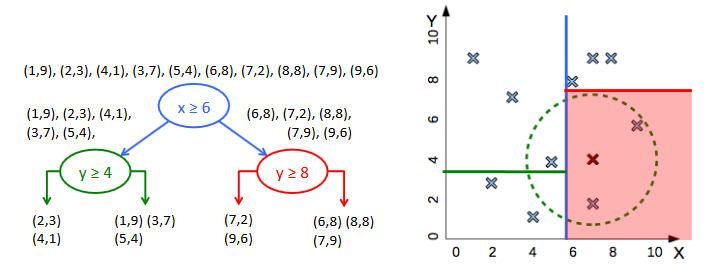
\includegraphics[width=\linewidth,keepaspectratio]{knn7}
%\end{center}
%\end{frame}
%
%
%
%%%%%%%%%%%%%%%%%%%%%%%%%%%%%%%%%%%%%%%%%%%%%%%%%%%%%%%%%%%
%\begin{frame}[fragile]\frametitle{Optimal Clustering}
%\begin{center}
%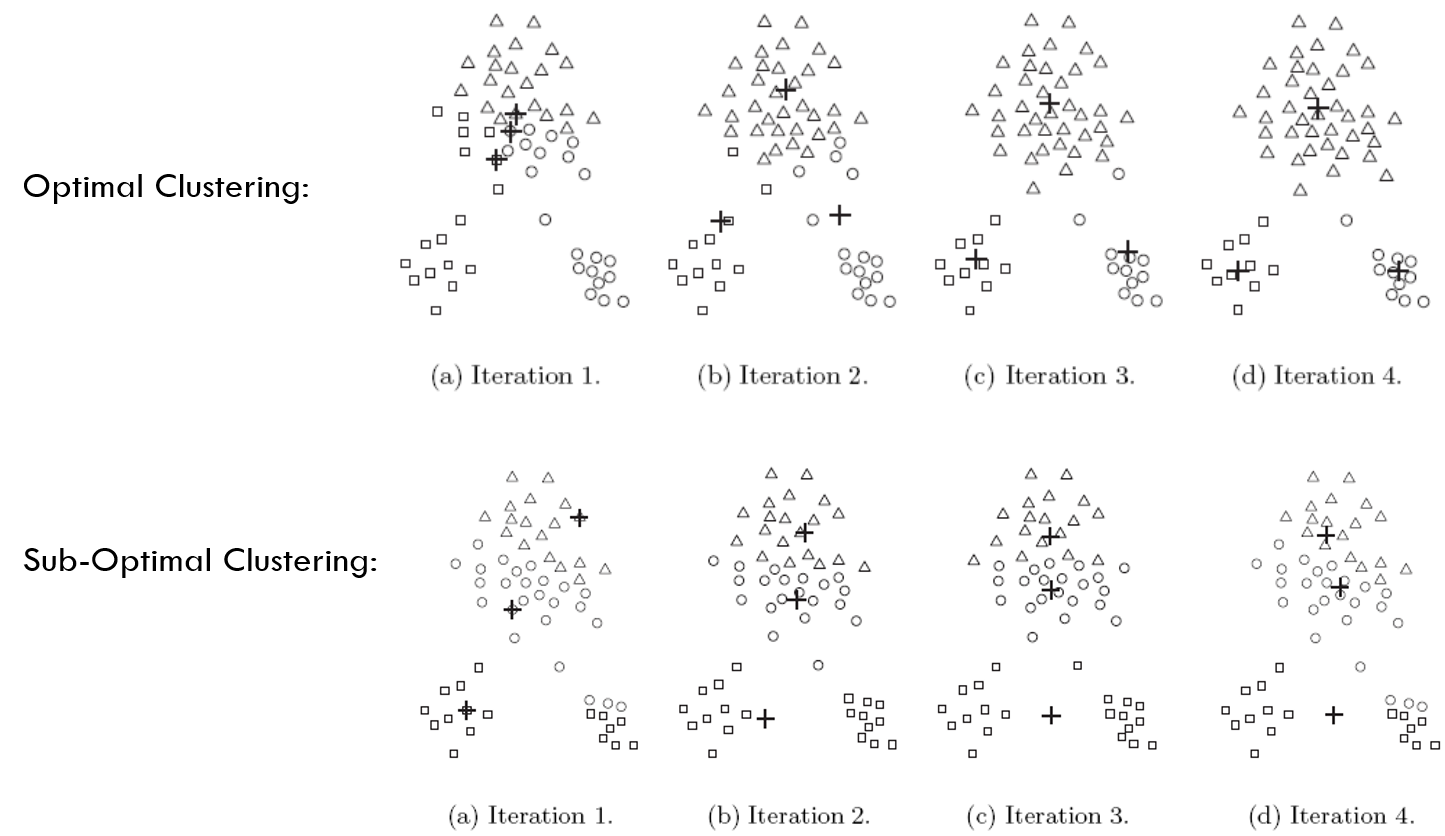
\includegraphics[width=\linewidth,keepaspectratio]{optiknn}
%\end{center}
%\end{frame}
%
%
%%%%%%%%%%%%%%%%%%%%%%%%%%%%%%%%%%%%%%%%%%%%%%%%%%%%%%%%%%%
%\begin{frame}[fragile]\frametitle{Partitioning}
%When k-NN is searching for the nearest neighbor, it is partitioning the abstract feature space into a Voronoi tessellation
%
%\begin{itemize}
%\item Each region belongs to an instance
%\item Contains all the points in the space whose distance to that instance is less than the distance to any other instance
%
%\end{itemize}
%\begin{center}
%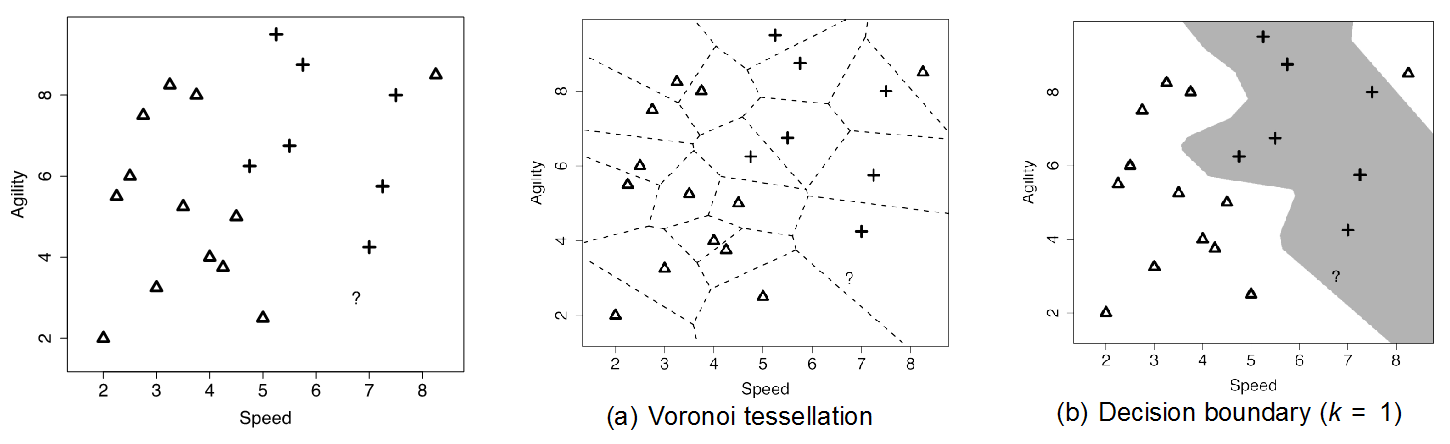
\includegraphics[width=0.6\linewidth,keepaspectratio]{voronoi}
%\end{center}
%\end{frame}
%
%%%%%%%%%%%%%%%%%%%%%%%%%%%%%%%%%%%%%%%%%%%%%%%%%%%%%%%%%%%
%\begin{frame}[fragile]\frametitle{K Nearest}
%One of the great things about nearest neighbor algorithms is that we can add in new data to update the model very easily. 
%
%
%\begin{itemize}
%\item Each region belongs to an instance
%\item Contains all the points in the space whose distance to that instance is less than the distance to any other instance
%
%\end{itemize}
%\begin{center}
%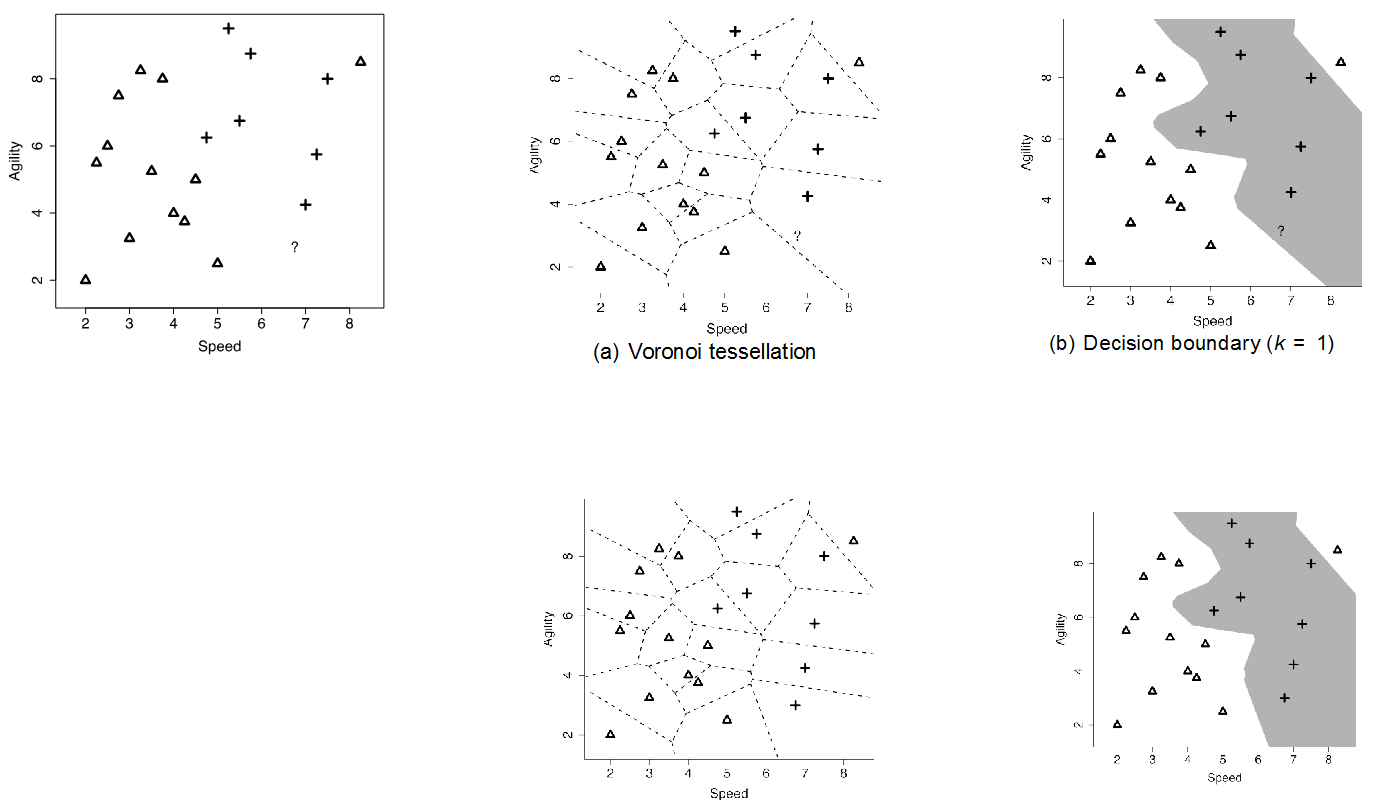
\includegraphics[width=0.6\linewidth,keepaspectratio]{knnnew}
%\end{center}
%\end{frame}
%
%%%%%%%%%%%%%%%%%%%%%%%%%%%%%%%%%%%%%%%%%%%%%%%%%%%%%%%%%%%
%\begin{frame}[fragile]\frametitle{Outliers}
%What's up with the top-right instance?
%
%\begin{itemize}
%\item Is it noise?
%\item The decision boundary is likely not ideal because of id13.
%\item k-NN is a set of local models, each defined by a single instance
%\item Sensitive to noise!
%\item How to mitigate noise?
%\item Choose a higher value of k.
%\end{itemize}
%\begin{center}
%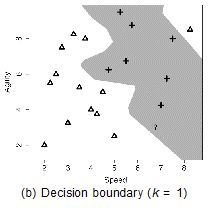
\includegraphics[width=0.4\linewidth,keepaspectratio]{knnout}
%\end{center}
%\end{frame}
%
%%%%%%%%%%%%%%%%%%%%%%%%%%%%%%%%%%%%%%%%%%%%%%%%%%%%%%%%%%%
%\begin{frame}[fragile]\frametitle{Different Values of k}
%Setting k to a high value is riskier with an imbalanced dataset.
%
%\begin{center}
%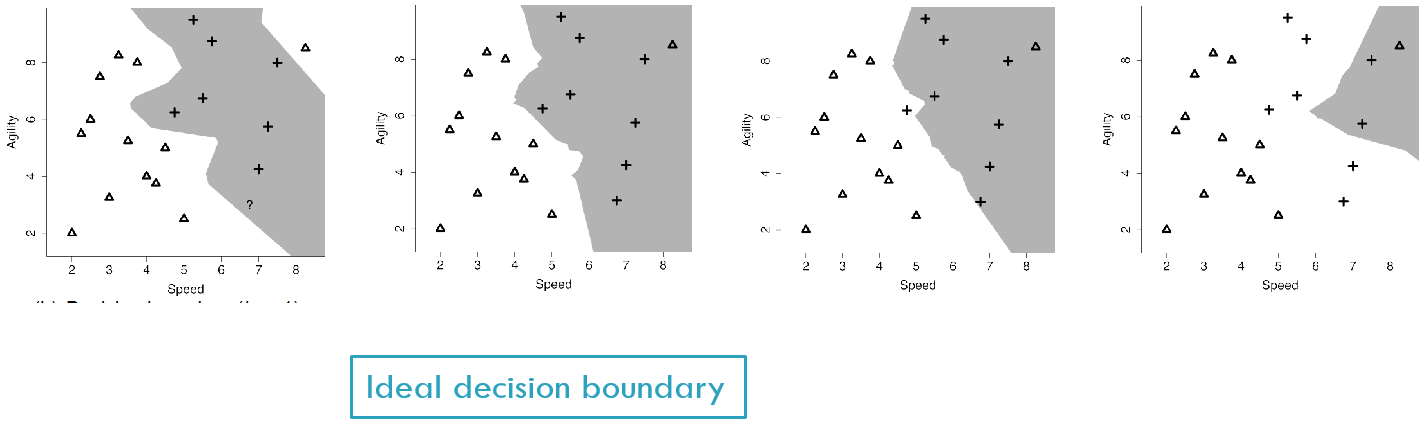
\includegraphics[width=\linewidth,keepaspectratio]{diffk}
%\end{center}
%Choose k by running evaluation experiments on a training or validation set.
%
%\end{frame}
%
%
%%%%%%%%%%%%%%%%%%%%%%%%%%%%%%%%%%%%%%%%%%%%%%%%%%%%
%\begin{frame}[fragile] \frametitle{Choosing the right k}
%
%\adjustbox{valign=t}{
%\begin{minipage}{0.45\linewidth}
%\begin{itemize}
%\item If k is too small, sensitive to noise points in the training data
%\item Susceptible to overfitting
%\item If k is too large, neighborhood may include points from other classes
%\item Susceptible to misclassification
%
%\end{itemize}
%
%\end{minipage}
%}
%\hfill
%\adjustbox{valign=t}{
%\begin{minipage}{0.45\linewidth}
%\begin{center}
%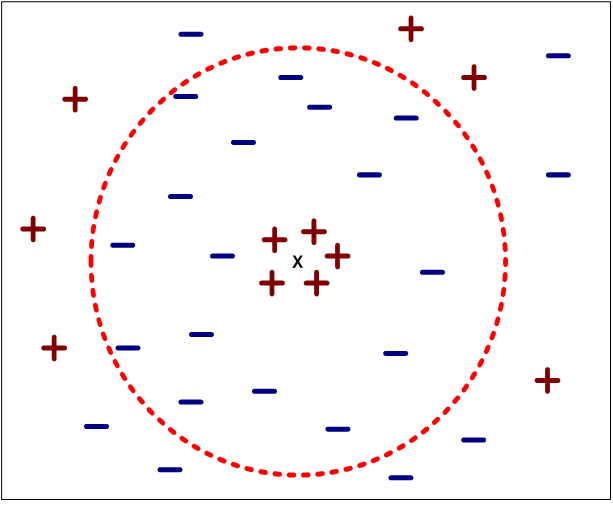
\includegraphics[width=\linewidth,keepaspectratio]{rightk}
%\end{center}
%
%\end{minipage}
%}
%\end{frame}


%%%%%%%%%%%%%%%%%%%%%%%%%%%%%%%%%%%%%%%%%%%%%%%%%%%%%%%%%%%%%%%%%%%%%%%%%%%%%%%%%%
\begin{frame}[fragile]\frametitle{}
\begin{center}
{\Large Summary}
\end{center}
\end{frame}

%%%%%%%%%%%%%%%%%%%%%%%%%%%%%%%%%%%%%%%%%%%%%%%%%%%%%%%%%%
\begin{frame}[fragile]\frametitle{Final Thoughts on Nearest Neighbors}
\begin{itemize}
\item Nearest-neighbors classification is part of a more general technique called instance-based learning
\item Use specific instances for prediction, rather than a model
\item Nearest-neighbors is a lazy learner
\item Performing the classification can be relatively computationally expensive
\item No model is learned up-front
\end{itemize}
\end{frame}

%%%%%%%%%%%%%%%%%%%%%%%%%%%%%%%%%%%%%%%%%%%%%%%%%%%%%%%%%%
\begin{frame}[fragile]\frametitle{Final Thoughts on Nearest Neighbors}
Pros
\begin{itemize}
\item The most attractive features of the K-nearest neighbor algorithm is that is simple to understand and easy to implement. 
\item With zero to little training time, it can be a useful tool for off-the-bat analysis of some data set you are planning to run more complex algorithms on. 
\item Furthermore, KNN works just as easily with multiclass data sets whereas other algorithms are hardcoded for the binary setting. 
\item Finally, as we mentioned earlier, the non-parametric nature of KNN gives it an edge in certain settings where the data may be highly ``unusual''.
\end{itemize}
\end{frame}

%%%%%%%%%%%%%%%%%%%%%%%%%%%%%%%%%%%%%%%%%%%%%%%%%%%%%%%%%%
\begin{frame}[fragile]\frametitle{Final Thoughts on Nearest Neighbors}
Cons
\begin{itemize}
\item Computationally expensive testing phase which is impractical in industry settings. 
\item Can suffer from skewed class distributions. For example, if a certain class is very frequent in the training set, it will tend to dominate the majority voting of the new example (large number = more common). 
\item Finally, the accuracy of KNN can be severely degraded with high-dimension data because there is little difference between the nearest and farthest neighbor.
\end{itemize}
\end{frame}


%%%%%%%%%%%%%%%%%%%%%%%%%%%%%%%%%%%%%%%%%%%%%%%%%%%%
%\begin{frame}[fragile] \frametitle{Classifier Comparison}
%
%\adjustbox{valign=t}{
%\begin{minipage}{0.45\linewidth}
%Eager Learners
%\begin{itemize}
%\item Decision Trees, SVMs
%\item Model Building: potentially slow 
%\item Classifying Test Instance: fast
%\item finding a global model that fits the entire input space
%
%\end{itemize}
%
%\end{minipage}
%}
%\hfill
%\adjustbox{valign=t}{
%\begin{minipage}{0.45\linewidth}
%Lazy Learners
%\begin{itemize}
%\item Nearest Neighbors
%\item Model Building: fast (because there is none!)
%\item Classifying Test Instance: slow
%\item classification decisions are made locally (small k values), and are more susceptible to noise
%\end{itemize}
%
%\end{minipage}
%}
%\end{frame}

%%%%%%%%%%%%%%%%%%%%%%%%%%%%%%%%%%%%%%%%%%%%%%%%%%%%%%%%%%
\begin{frame}[fragile]\frametitle{K- Nearest Neighbors (Recap)}
\begin{itemize}
\item k = parameter, chosen by analyst
\item For a given test instance, use the k ``closest'' points (nearest neighbors) for performing classification
\item ``closest'' points: defined by some proximity metric, such as Euclidean Distance
\item Requires three things
	\begin{itemize}
	\item The set of stored records
	\item Distance Metric to compute distance between records
	\item The value of k, the number of nearest neighbors to retrieve
	\end{itemize}
\end{itemize}
\end{frame}




%%%%%%%%%%%%%%%%%%%%%%%%%%%%%%%%%%%%%%%%%%%%%%%%%%%%
%\begin{frame}[fragile] \frametitle{}
%Here is an example dataset that we will use:
%\begin{center}
%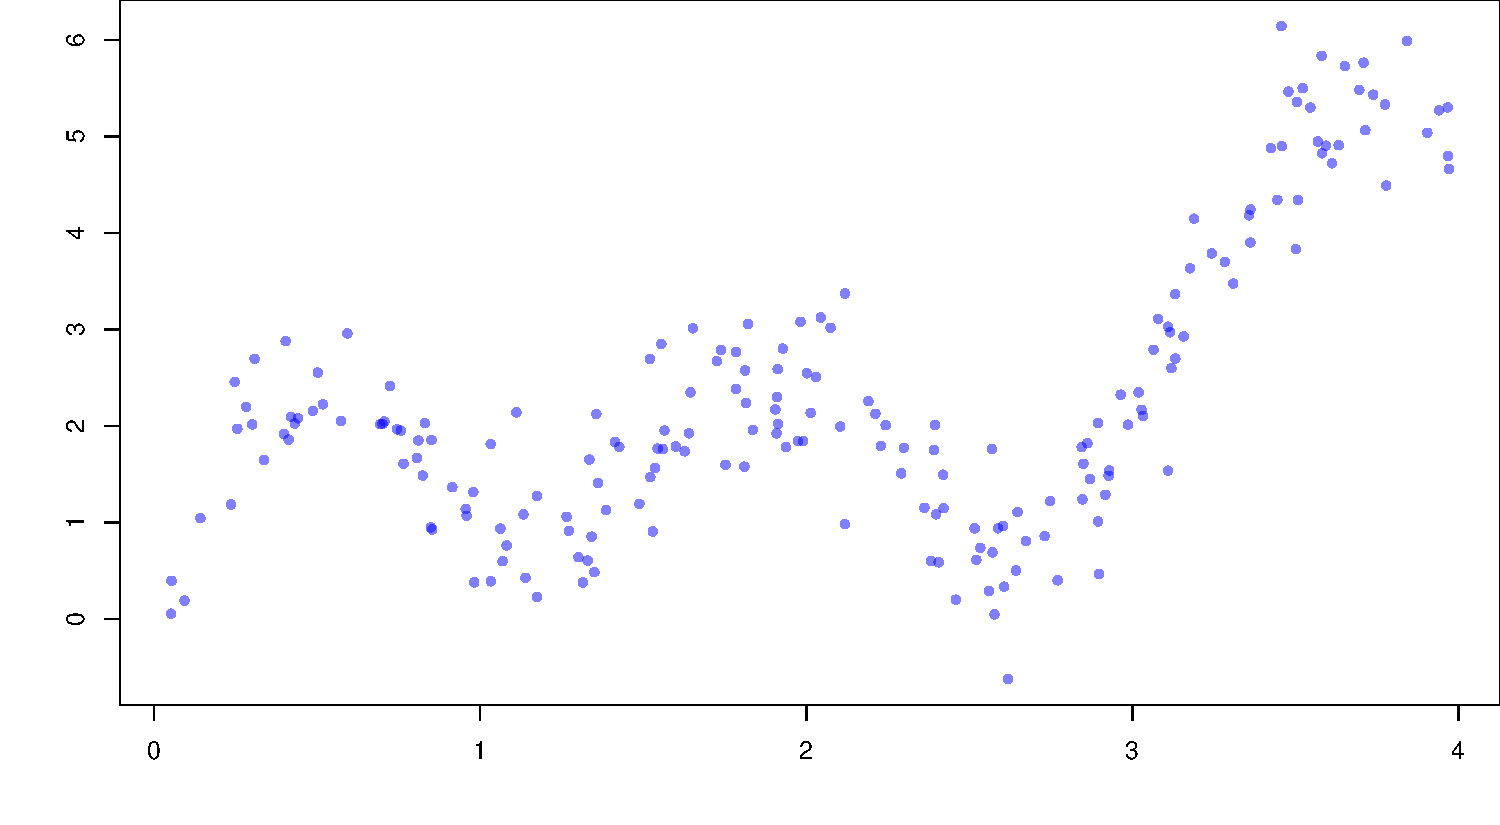
\includegraphics[width=0.5\linewidth]{scatter.pdf}
%\end{center}
%One of the most straightforward estimators, knn simply sets $\widehat{g}(x_{new})$ to be
%the average value of the observed $y$ of the $k$ closest points $x_j$ to $x_{new}$.
%\end{frame}
%
%%%%%%%%%%%%%%%%%%%%%%%%%%%%%%%%%%%%%%%%%%%%%%%%%%%%
%\begin{frame}[fragile] \frametitle{k-Nearest neighbors (knn)}
%
%
%\begin{center}
%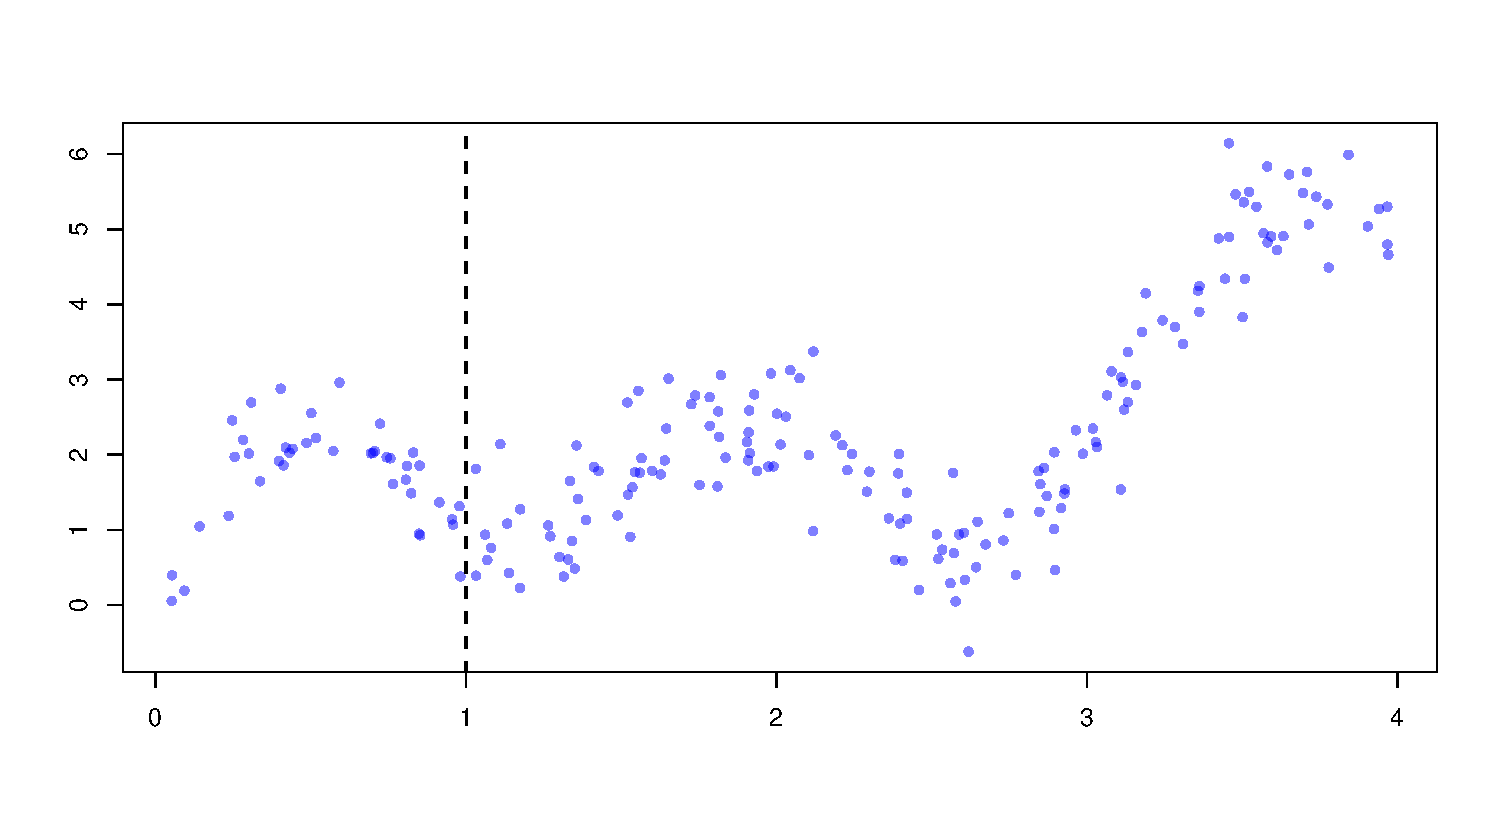
\includegraphics[width=0.5\linewidth]{knn1.pdf}
%\end{center}
%
%\begin{center}
%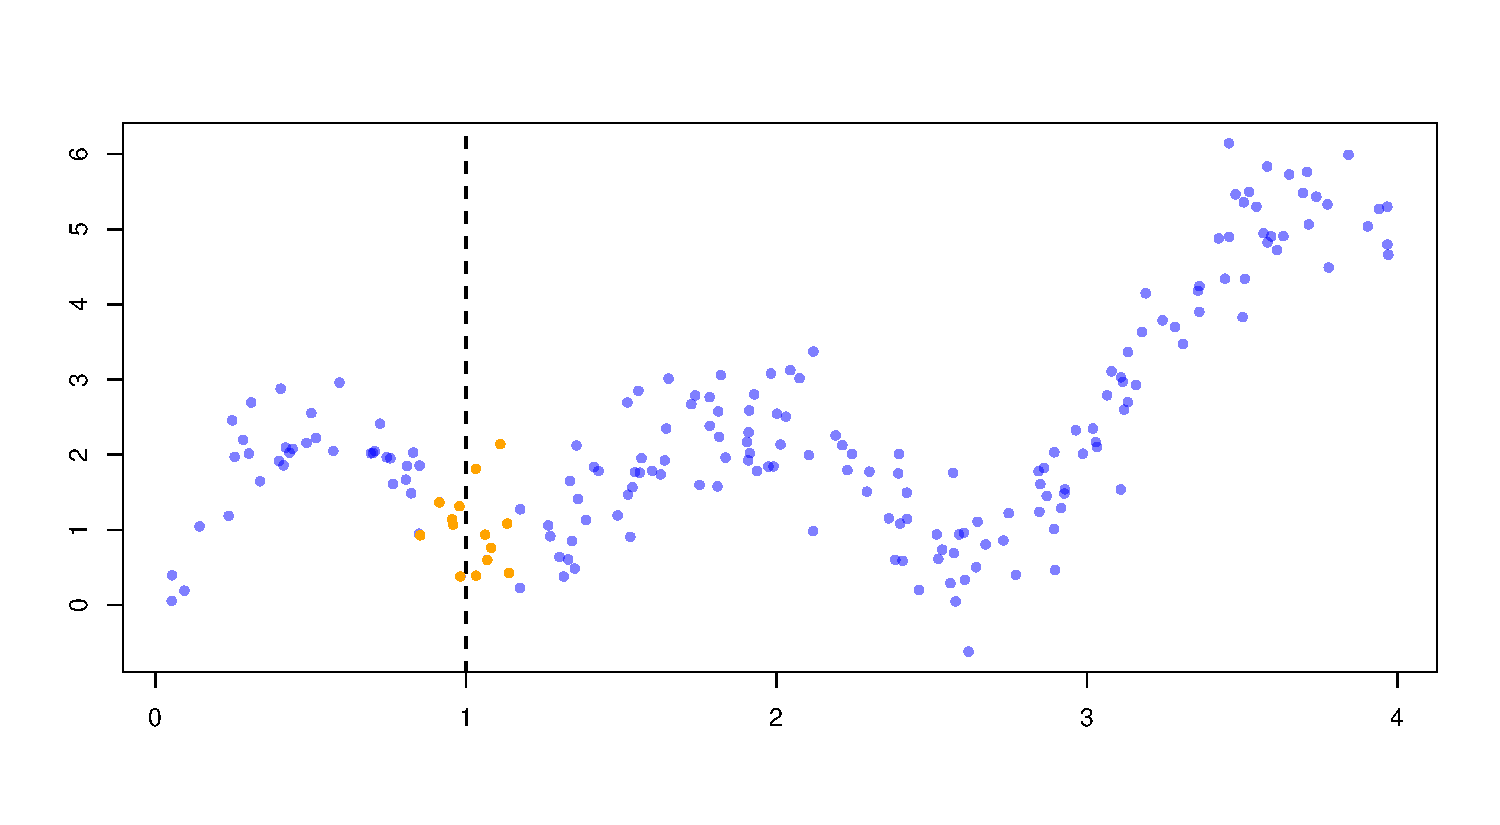
\includegraphics[width=0.5\linewidth]{knn2.pdf}
%\end{center}
%\end{frame}
%
%%%%%%%%%%%%%%%%%%%%%%%%%%%%%%%%%%%%%%%%%%%%%%%%%%%%
%\begin{frame}[fragile] \frametitle{}
%\begin{center}
%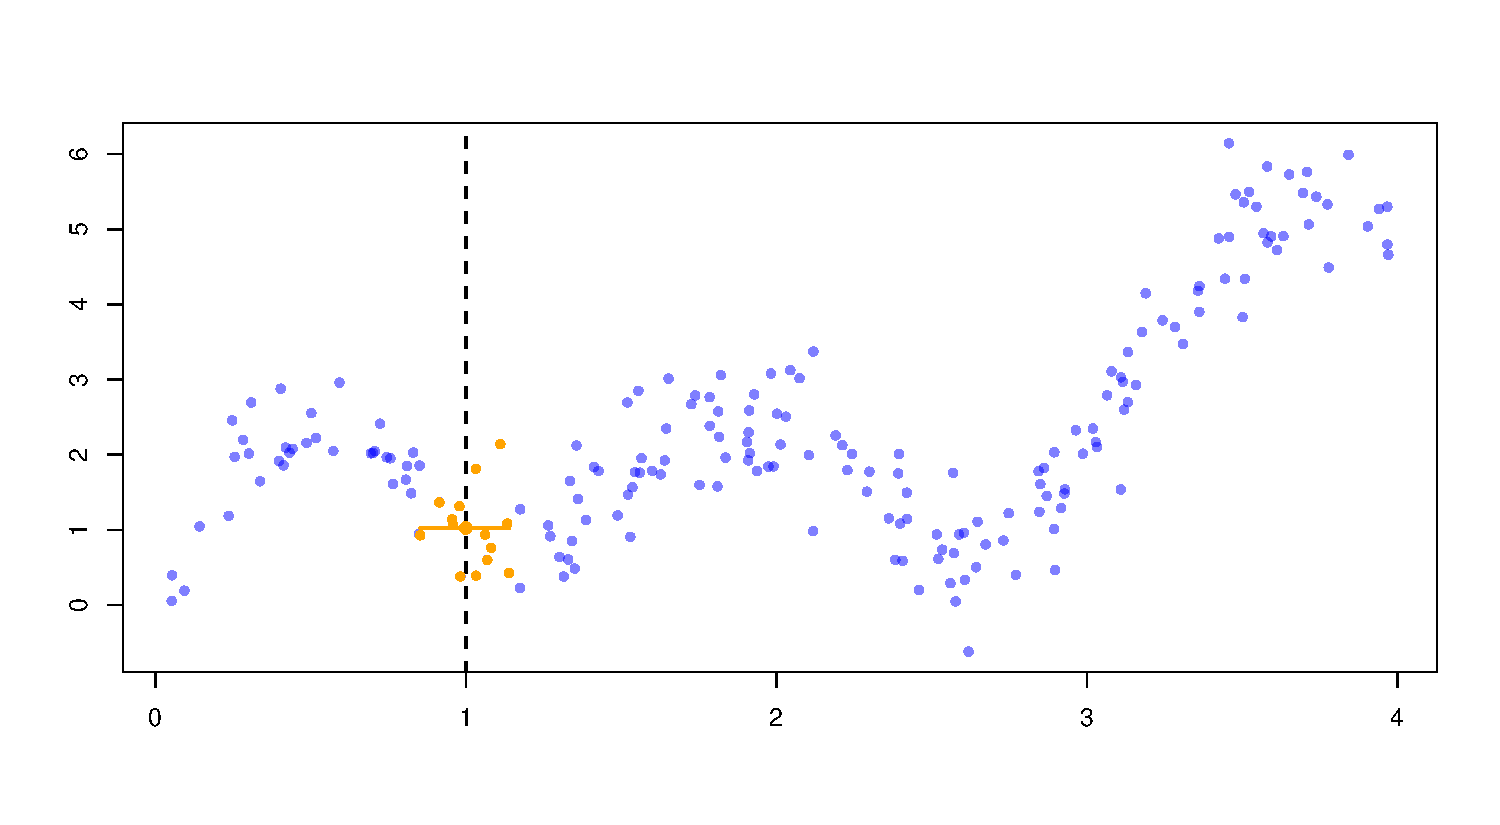
\includegraphics[width=0.5\linewidth]{knn3.pdf}
%\end{center}
%
%\begin{center}
%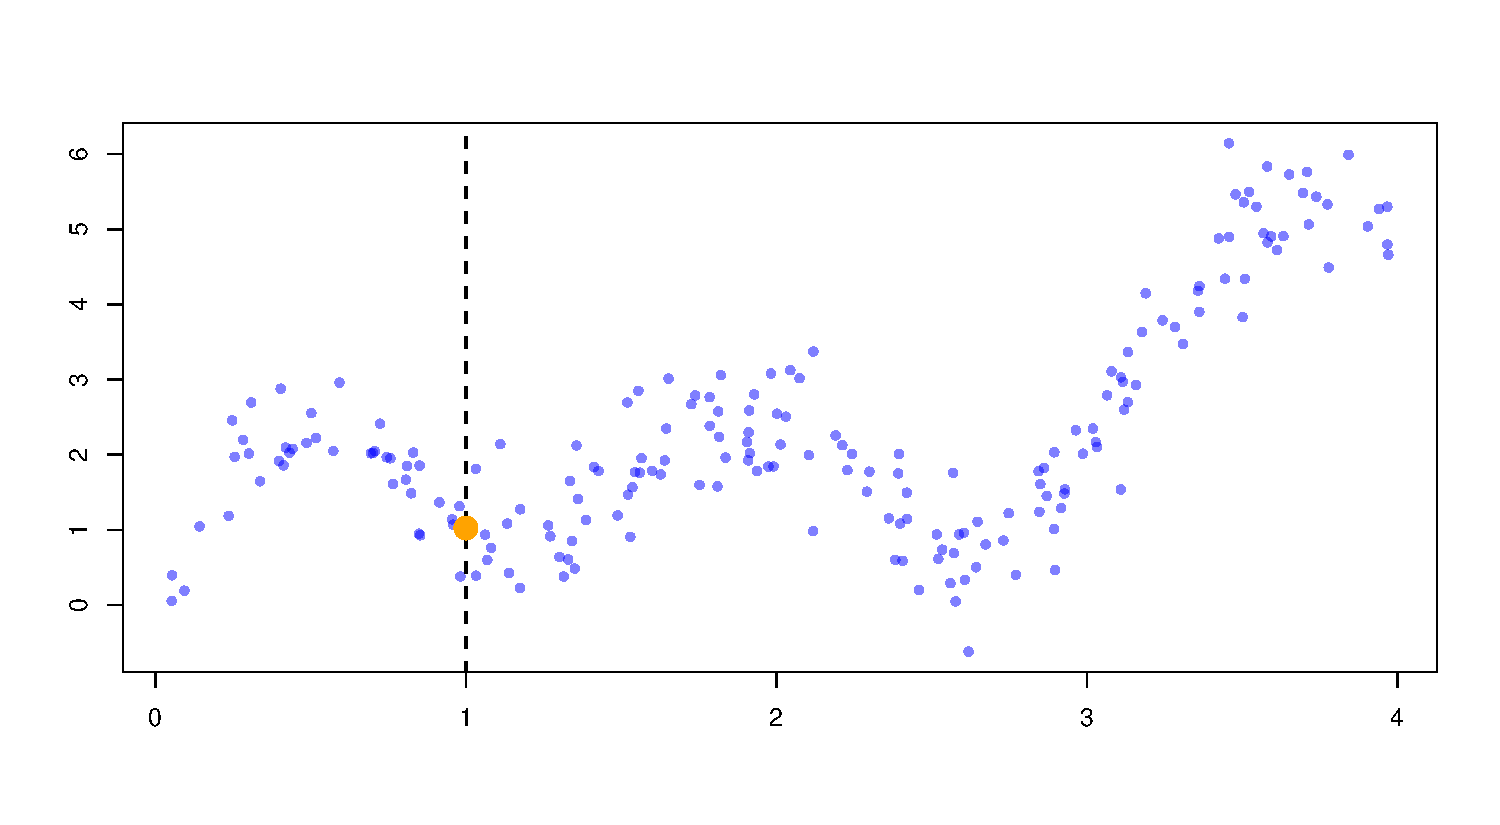
\includegraphics[width=0.5\linewidth]{knn4.pdf}
%\end{center}
%\end{frame}
%
%%%%%%%%%%%%%%%%%%%%%%%%%%%%%%%%%%%%%%%%%%%%%%%%%%%%
%\begin{frame}[fragile] \frametitle{k-Nearest neighbors (knn)}
%\begin{itemize}
%\item How might you expect the optimal parameter $k$ to change as $n$ increases?
%\item Rather than averaging the $k$-closest points, kernel smoothers average
%observations in the dataset using weights that are inversely proportional
%to the distance from the prediction point.
%\end{itemize}
%\end{frame}
%
%%%%%%%%%%%%%%%%%%%%%%%%%%%%%%%%%%%%%%%%%%%%%%%%%%%%
%\begin{frame}[fragile] \frametitle{Kernel smoothers}
%As an example, consider this estimator
%\begin{align*}
%\widehat{g}(x_{new}) &= \frac{\sum_i y_i \cdot \phi(||x_i - x_{new}||_2^2) }{\sum_i \phi(||x_i - x_{new}||_2^2)}
%\end{align*}
%Where $\phi$ is defined as the density function of a standard normal distribution:
%\begin{align*}
%\phi(z) &= \frac{1}{\sqrt{2\pi}} e^{-z^2/2}
%\end{align*}
%
%The function $\phi$ can be replaced with any other function that you
%would like to use. It is often replaced by a truncated variant, as
%observations more than a few standard deviations do not give a
%noticeable impact on the result.
%\end{frame}
%
%%%%%%%%%%%%%%%%%%%%%%%%%%%%%%%%%%%%%%%%%%%%%%%%%%%%
%\begin{frame}[fragile] \frametitle{Kernel smoothers  - bandwidth}
%What is the main tuning parameter for kernel smoothers? We need to modify
%our estimator slightly to include the {\bf bandwidth} parameter $h$:
%\begin{align*}
%\widehat{g}(x_{new}) &= \frac{\sum_i y_i \cdot \phi(||x_i - x_{new}||_2^2 / h) }{\sum_i \phi(||x_i - x_{new}||_2^2 / h)}
%\end{align*}
%What does the bandwidth control?
% Why might we think of the bandwidth as a standard deviation?
%
%\begin{center}
%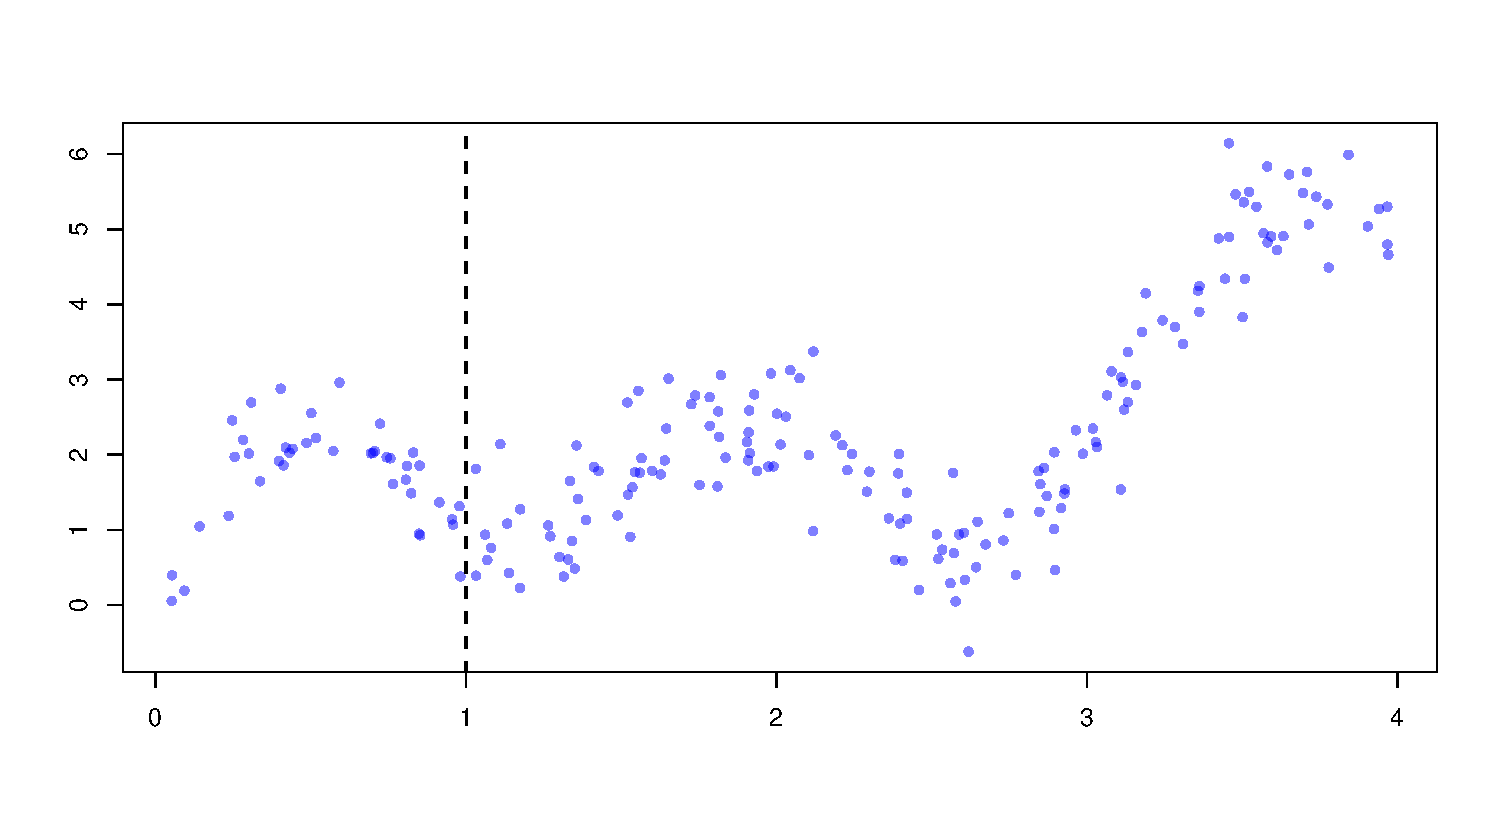
\includegraphics[width=0.5\linewidth]{ksmooth1.pdf}
%\end{center}
%\end{frame}
%
%%%%%%%%%%%%%%%%%%%%%%%%%%%%%%%%%%%%%%%%%%%%%%%%%%%%
%\begin{frame}[fragile] \frametitle{}
%\begin{center}
%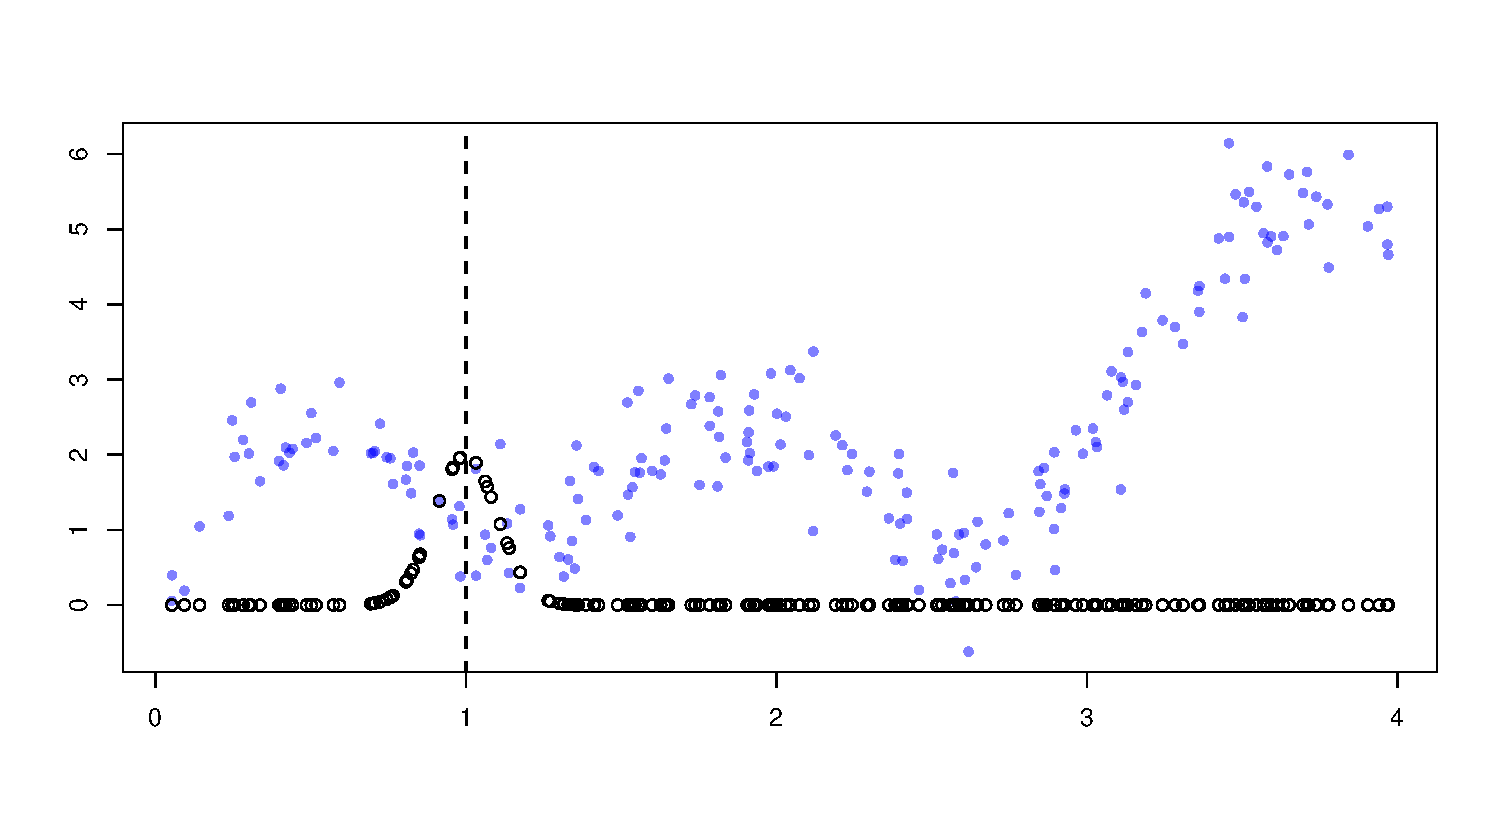
\includegraphics[width=0.5\linewidth]{ksmooth2.pdf}
%\end{center}
%
%\begin{center}
%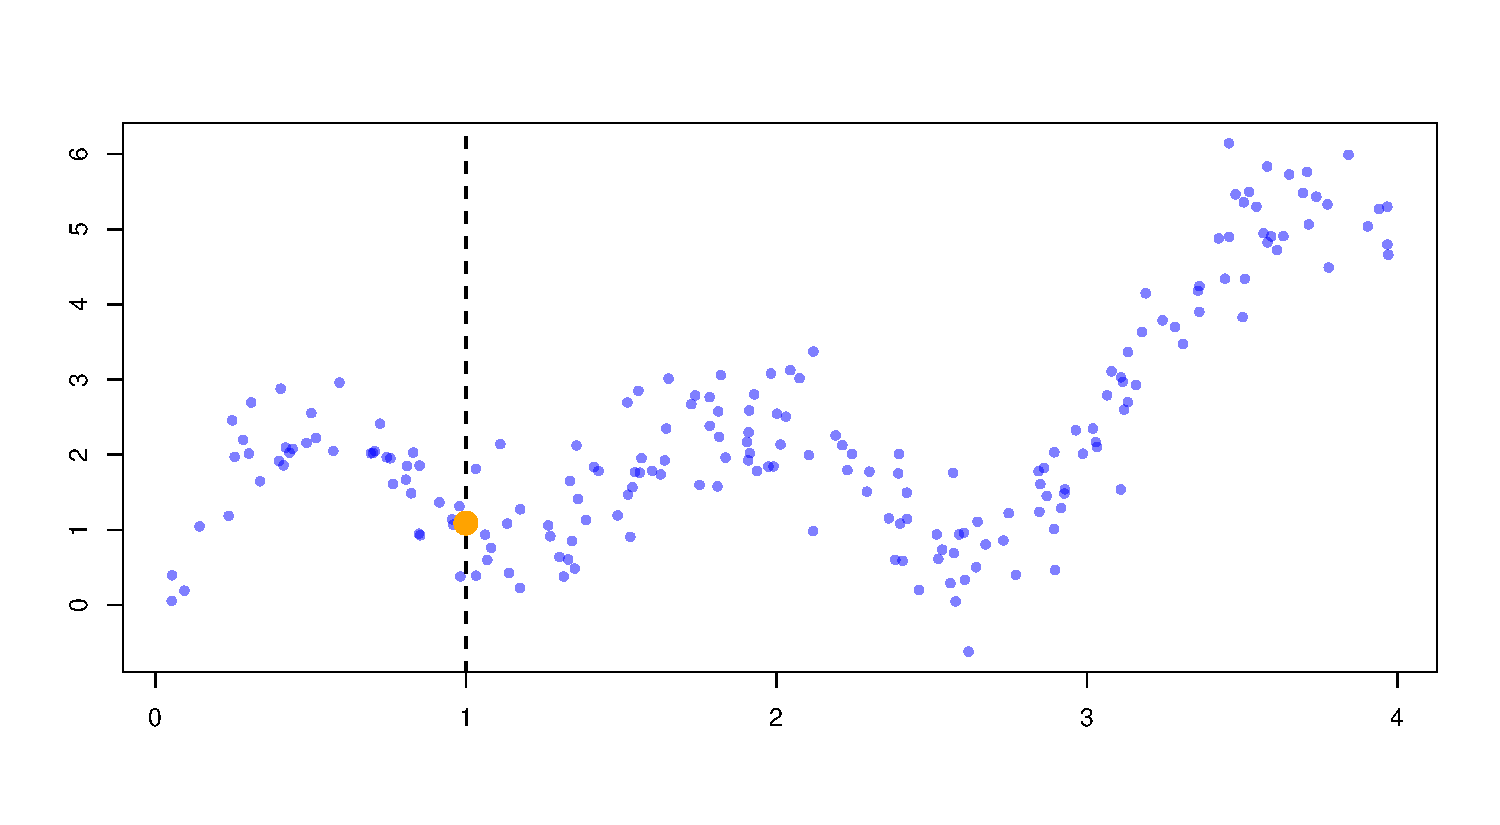
\includegraphics[width=0.5\linewidth]{ksmooth3.pdf}
%\end{center}
%\end{frame}
%
